\documentclass[12pt]{article}
\usepackage{homework}

\onehalfspacing
\graphicspath{{images/}}
\geometry{letterpaper, portrait, includeheadfoot=true, hmargin=1in, vmargin=1in}

\setcounter{section}{-1}
%%%%%%%%%%%%%%%%%%%%%%%%%%%%%%%%%%%%
%% Solution hiding %%
\usepackage[utf8]{inputenc}
\usepackage{lipsum}

\usepackage{ifthen}
\newboolean{hidesoln}
\setboolean{hidesoln}{false} 
\newboolean{hiderubric}
\setboolean{hiderubric}{false}
%%%%%%%%%%%%%%%%%%%%%%%%%%%%%%%%%%%%

% following loops stolen from djhsu
\def\ddefloop#1{\ifx\ddefloop#1\else\ddef{#1}\expandafter\ddefloop\fi}
\def\ddef#1{\expandafter\def\csname bb#1\endcsname{\ensuremath{\mathbb{#1}}}}
\ddefloop ABCDEFGHIJKLMNOPQRSTUVWXYZ\ddefloop
\def\ddef#1{\expandafter\def\csname c#1\endcsname{\ensuremath{\mathcal{#1}}}}
\ddefloop ABCDEFGHIJKLMNOPQRSTUVWXYZ\ddefloop
\def\ddef#1{\expandafter\def\csname bf#1\endcsname{\ensuremath{\mathbf{#1}}}}
\ddefloop ABCDEFGHIJKLMNOPQRSTUVWXYZabcdefghijklmnopqrstuvwxyz\ddefloop
% \cA, \cB, ...
\def\ddef#1{\expandafter\def\csname c#1\endcsname{\ensuremath{\mathcal{#1}}}}
\ddefloop ABCDEFGHIJKLMNOPQRSTUVWXYZ\ddefloop

% \vA, \vB, ..., \va, \vb, ...
\def\ddef#1{\expandafter\def\csname v#1\endcsname{\ensuremath{\boldsymbol{#1}}}}
\ddefloop ABCDEFGHIJKLMNOPQRSTUVWXYZabcdefghijklmnopqrstuvwxyz\ddefloop
% \valpha, \vbeta, ...,  \vGamma, \vDelta, ...,
\def\ddef#1{\expandafter\def\csname v#1\endcsname{\ensuremath{\boldsymbol{\csname #1\endcsname}}}}
\ddefloop {alpha}{beta}{gamma}{delta}{epsilon}{varepsilon}{zeta}{eta}{theta}{vartheta}{iota}{kappa}{lambda}{mu}{nu}{xi}{pi}{varpi}{rho}{varrho}{sigma}{varsigma}{tau}{upsilon}{phi}{varphi}{chi}{psi}{omega}{Gamma}{Delta}{Theta}{Lambda}{Xi}{Pi}{Sigma}{varSigma}{Upsilon}{Phi}{Psi}{Omega}{ell}\ddefloop

\def\SPAN{\textup{span}}
\def\tu{\textup{u}}
\def\R{\mathbb{R}}
\def\E{\mathbb{E}}
\def\Z{\mathbb{Z}}
\def\be{\mathbf{e}}
\def\nf{\nabla f}
\def\veps{\varepsilon}
\def\cl{\textup{cl}}
\def\inte{\textup{int}}
\def\dom{\textup{dom}}
\def\Rad{\textup{Rad}}
\def\lsq{\ell_{\textup{sq}}}
\def\hcR{\widehat{\cR}}
\def\hcRl{\hcR_\ell}
\def\cRl{\cR_\ell}
\def\hcE{\widehat{\cE}}
\def\cEl{\cE_\ell}
\def\hcEl{\hcE_\ell}
\def\eps{\epsilon}
\def\1{\mathds{1}}
\newcommand{\red}[1]{{\color{red} #1}}
\newcommand{\blue}[1]{{\color{blue} #1}}
\def\srelu{\sigma_{\textup{r}}}
\def\vsrelu{\vec{\sigma_{\textup{r}}}}
\def\vol{\textup{vol}}
\def\tF{{\scriptscriptstyle\textup{F}}}
\DeclareMathOperator{\tr}{tr}
\newcommand\T{{\scriptscriptstyle\mathsf{T}}}

\newcommand{\ip}[2]{\left\langle #1, #2 \right \rangle}
\newcommand{\mjt}[1]{{\color{blue}\emph\textbf{[M:}~#1~\textbf{]}}}

\def\hPr{\widehat{\textup{Pr}}}
\def\Lip{\textup{Lip}}

\begin{document}
\singlespacing

\renewcommand{\familydefault}{\rmdefault}
\pagestyle{fancy}
\fancyhf{}
\setlength{\headheight}{30pt}
\renewcommand{\headrulewidth}{0.4pt}
\renewcommand{\footrulewidth}{0.4pt}
\lhead{\large Homework 2 \\ Due Feb. 20, 2024 }
\rhead{\large CS 446 \\ Spring 2024}
\rfoot{\textbf{Page \thepage}}
\lfoot{}

\section{Instructions}

Homework is due Tuesday, April 2, 2024 at 23:59pm Central Time.
Please refer to \url{https://courses.grainger.illinois.edu/cs446/sp2024/homework/hw/index.html} for course policy on homeworks and submission instructions.

\ifthenelse{\boolean{hidesoln}}{}{
    \textbf{Reminder:} Answers must be typeset. \LaTeX  and other methods of typesetting math are accepted.
}

\section{PCA: 6pts}
\begin{enumerate}

\item According to the definition of PCA, the first principal component of $w$ is the one that makes the variance of the projected data $Xw$ the largest. In this case, the direction of $w$ is the line cross both data points (see Figuere 1), i.e. $w = (\frac{3}{5} ,  \frac{4}{5})^T $.
\begin{figure}[H]
    \centering
    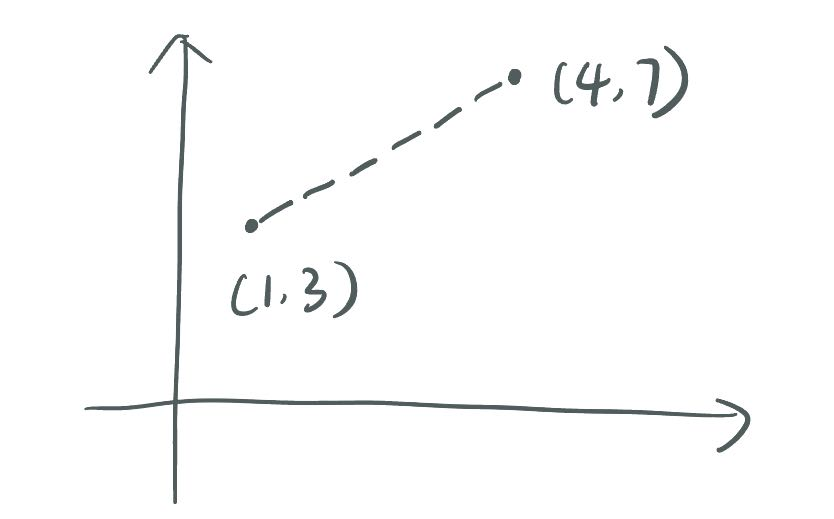
\includegraphics[width=0.4\textwidth]{../img/q1-1.jpg}
    \caption{Q 1.1}
\end{figure}

\item \begin{figure}[H]
    \centering
    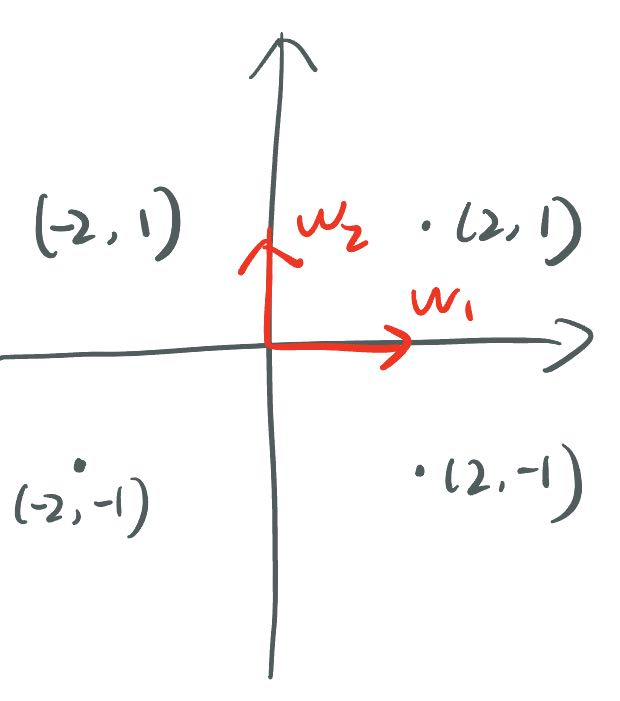
\includegraphics[width=0.3\textwidth]{../img/q1-2.jpg}
    \caption{Q 1.2}
\end{figure}
\begin{align}
    \mu = \frac{1}{4} \sum x_i = (1, 4)^T \nonumber
\end{align}
Then, we get the centralized data (as shown in Figure 2).
\begin{align}
    X = \begin{bmatrix}
        -2 & -2 & 2 & 2 \\
        -1 & 1 & -1 & 1
    \end{bmatrix} \nonumber
\end{align}

The covariance matrix is, 
\begin{align}
    \Sigma = \frac{1}{3} X X^T = \begin{bmatrix}
        \frac{16}{3} & 0  \\
        0 & \frac{4}{3}
    \end{bmatrix} \nonumber
\end{align}

We know that the first and second principal components are corresponding to the first and second largest eigenvalues of $\Sigma$. 

Because $\Sigma$ is diagonal, the largest eigenvalue is $\frac{16}{3}$ and the corresponding eigenvector is $(1, 0)^T$. 

The second largest eigenvalue is $\frac{4}{3}$ and the corresponding eigenvector is $(0, 1)^T$.

Therefore, the first and second principal components are $(1, 0)^T$ and $(0, 1)^T$ respectively.

\item $w^T \Sigma w$ is in a quadratic form. Because $\Sigma$ is diagonal, the quadratic form only contains squared terms.
Under the constraint $w^T w = 1$, we have,
\begin{eqnarray}
    w^T \Sigma w &=& 12 w_1^2 + 6 w_2^2 + 20 w_3^2 + 10 w_4^2 \nonumber\\
                &\le& 20 \nonumber\\
\end{eqnarray}
$w^T \Sigma w = 20$ only when $w = [0, 0, 1, 0]^T$. Therefore, the optimal $w$ is $[0, 0, 1, 0]^T$.

\end{enumerate}
    
\section{Basics in Information Theory: 7pts}

\begin{enumerate}
    \item \begin{eqnarray}
        Pr(X' = x) &=& Pr(X' = x|B = 1)Pr(B = 1) + Pr(X' = x|B = 0) Pr(B = 0) \nonumber \\ 
        &=& Pr(X = x) \lambda + Pr(X = x) (1-\lambda)\nonumber\\
    \end{eqnarray}

    \item \begin{eqnarray}
        D_{\lambda}(P || Q) &=& \lambda D_{KL}(P || \lambda P + (1- \lambda) Q) + (1-\lambda) D_{KL}(Q || \lambda P + (1- \lambda) Q) \nonumber \\ 
        &=& \lambda \int p(x) \log \frac{p(x)}{\lambda p(x) + (1-\lambda) q(x)}\,dx + (1-\lambda) \int q(x) \log \frac{q(x)}{\lambda p(x) + (1-\lambda) q(x)}\,dx \nonumber\\ 
        &=& \lambda \int p(x) (\log p(x) - \log (\lambda p(x) + (1-\lambda)q(x))) \,dx \nonumber\\ 
        && + (1-\lambda) \int q(x) (\log q(x) - \log (\lambda p(x) + (1-\lambda)q(x))) \,dx \nonumber\\
        &=& -\int (\lambda p(x) + (1-\lambda)q(x)) \log (\lambda p(x) +  (1-\lambda)q(x)) \,dx  \nonumber\\
        && + \lambda \int p(x) \log p(x) \,dx + (1-\lambda) \int q(x) \log q(x) \,dx \nonumber\\ 
        &=& H(X') - \lambda H(X'|B = 1) - (1-\lambda) H(X' | B = 0) \nonumber\\
        &=& H(X') - H(X' | B)\nonumber\\ \nonumber
        &=& I(X'; B)
    \end{eqnarray}
\end{enumerate}

\section{k-Means with Soft Assignments: 10pts}

\begin{enumerate}
    \item 
    \begin{align}
        \underset{\mu_1, ..., \mu_K}{\min}\underset{\substack{A \in [0,1]^{n\times K} \\ A\cdot\mathbf{1}_K= \mathbf{1}_n}}{\min}\sum_{i=1}^n\sum_{k=1}^K A_{ik}\|x^{(i)} - \mu_k\|^2_2 \leq \underset{\mu_1, ..., \mu_K}{\min}\underset{\substack{A \in \{0,1\}^{n\times K} \\ A\cdot\mathbf{1}_K= \mathbf{1}_n}}{\min}\sum_{i=1}^n\sum_{k=1}^K A_{ik}\|x^{(i)} - \mu_k\|^2_2\notag
    \end{align} 
    Because the right side is minimizing over a subset of feasible $A$ of right side. Therefore, for every optimal $A*$ on the right side, we can always find the same $A*$ on the left side. Therefore, the left side is less than or equal to the right side.

    \item 
    \begin{align}
        \underset{\mu_1, ..., \mu_K}{\min}\underset{\substack{A \in [0,1]^{n\times K} \\ A\cdot\mathbf{1}_K= \mathbf{1}_n}}{\min}\sum_{i=1}^n\sum_{k=1}^K A_{ik}\|x^{(i)} - \mu_k\|^2_2 \geq \underset{\mu_1, ..., \mu_K}{\min}\underset{\substack{A \in \{0,1\}^{n\times K} \\ A\cdot\mathbf{1}_K= \mathbf{1}_n}}{\min}\sum_{i=1}^n\sum_{k=1}^K A_{ik}\|x^{(i)} - \mu_k\|^2_2\notag
    \end{align}
    
    Suppose $mu_{l^*}$ is the solution of $mu_l$ to $\|x^{(i)} - \mu_k\|^2_2 \geq \underset{l}{\min}\|x^{(i)} - \mu_l\|^2_2$. Then for any $A \in [0,1]^{n\times K}$, we have,
    \begin{eqnarray}
        \sum_{k=1}^K A_{ik}||x^{(i)} - \mu_k||^2_2 &\geq& \sum_{k=1}^K A_{ik}||x^{(i)} - \mu_{l^*}||^2_2 \nonumber\\
        &=& (\sum_{k=1}^K A_{ik})||x^{(i)} - \mu_{l^*}||^2_2 \nonumber\\
        &=& ||x^{(i)} - \mu_{l^*}||^2_2 \nonumber \\
        &=& \underset{\substack{A \in \{0,1\}^{n\times K} \\ A\cdot\mathbf{1}_K= \mathbf{1}_n}}{\min} \sum_{k=1}^K A_{ik} ||x^{(i)} - \mu_{k}||^2_2 \nonumber
    \end{eqnarray}
    Thus, for the optimal $A$ that makes the left side minimum, the above inequality still holds, i.e.,
    \begin{align}
        \underset{\substack{A \in [0,1]^{n\times K} \\ A\cdot\mathbf{1}_K= \mathbf{1}_n}}{\min} \sum_{k=1}^K A_{ik} ||x^{(i)} - \mu_{k}||^2_2 \geq \underset{\substack{A \in \{0,1\}^{n\times K} \\ A\cdot\mathbf{1}_K= \mathbf{1}_n}}{\min} \sum_{k=1}^K A_{ik} ||x^{(i)} - \mu_{k}||^2_2 \nonumber
    \end{align} Thus, the original inequality also holds.

    \item From the above two question, we know that the left side and the right side are equal. In other words, the optimal solution to soft assignment problem is equal to the optimal solution to hard assignment problem.
    
\end{enumerate}


\section{Bernoulli Mixture Model: 18pts}
Suppose the k-th element of $z_i$ is 1, then the likelihood is,
\begin{enumerate}
    \item \begin{eqnarray}
        \Pr(x^{(i)}, z_i| \pi, \mu) &=& \Pr(x^{(i)}|z_ik = 1) \Pr(z_ik = 1) \nonumber\\
        &=& \Pr(x^{(i)}|\mu_k) \pi_k \nonumber\\
        &=& \pi_k \prod_{j=1}^d \mu_{k}^{x^{(i)}_j} (1-\mu_k)^{1-x^{(i)}_j} \nonumber \\
    \end{eqnarray}

    Thus, the log-likelihood is,
    \begin{eqnarray}
        \log\Pr(x^{(i)}, z_i| \pi, \mu) &=&  \log \pi_k + \sum_{j=1}^d \mu_{k}^{x^{(i)}_j} (1-\mu_k)^{1-x^{(i)}_j} \nonumber\\
        &=& \log \pi_k + \sum_{j=1}^d x^{(i)}_j \log \mu_k + \sum_{j=1}^d (1-x^{(i)}_j) \log (1-\mu_k) \nonumber
    \end{eqnarray}

    \item \begin{eqnarray}
        Pr(z_{ik} = 1 | x^{(i)}) &=& \frac{Pr(x^{(i)}|z_{ik} = 1) Pr(z_{ik} = 1)}{\sum_{k=1}^K Pr(x^{(i)}| z_i) Pr(z_{ik} = 1)} \nonumber\\
        &=& \frac{\pi_k \prod_{j=1}^d \mu_{k}^{x^{(i)}_j} (1-\mu_k)^{1-x^{(i)}_j}}{\sum_{k=1}^K \pi_k \prod_{j=1}^d \mu_{k}^{x^{(i)}_j} (1-\mu_k)^{1-x^{(i)}_j}} \nonumber
    \end{eqnarray}
    \item \begin{eqnarray}
        \min -\log \prod_{i \in D} p(x^{i} | \mu, \pi) & = & \min -\sum_{i \in D} \log p(x^{i} | \mu, \pi) \nonumber\\
        & = & \min -\sum_{i \in D} \log \sum_{k=1}^K \pi_k \prod_{j=1}^d \mu_{k}^{x^{(i)}_j} (1-\mu_k)^{1-x^{(i)}_j} \nonumber
    \end{eqnarray}
    Take the derivative with respect to $\mu_k$ and $\pi_k$ , we have,
    \begin{eqnarray}
        \frac{d}{d \mu_k} &=& -\sum_{i \in D} \frac{( \pi_k \prod_{j=1}^{d} \mu_k ^{x_j^{(i)}} (1-\mu_k)^{(1 - x_j^{(i)})} )'}{ \sum_{k=1}^K \pi_k \prod_{j=1}^d \mu_{k}^{x^{(i)}_j} (1-\mu_k)^{1-x^{(i)}_j} } \nonumber
        \\ &=& -\sum_{i \in D} \frac{( \pi_k \mu_k ^{ \sum_{j=1}^{d} x_j^{(i)} } (1-\mu_k)^{ \sum_{j=1}^{d} (1 - x_j^{(i)})} )'}{ \sum_{k=1}^K \pi_k \prod_{j=1}^d \mu_{k}^{x^{(i)}_j} (1-\mu_k)^{1-x^{(i)}_j} } \nonumber
        \\ &=& -\sum_{i \in D} \frac{}{ \sum_{k=1}^K \pi_k \prod_{j=1}^d \mu_{k}^{x^{(i)}_j} (1-\mu_k)^{1-x^{(i)}_j} } \nonumber
        \\ &=& -\sum_{i \in D} \frac{ \pi_k (\sum_{j=1}^{d} x_j^{(i)}) \mu_k ^{ (\sum_{j=1}^{d} x_j^{(i)}) -1 } (1-\mu_k)^{ \sum_{j=1}^{d} (1 - x_j^{(i)})}}{ \sum_{k=1}^K \pi_k \prod_{j=1}^d \mu_{k}^{x^{(i)}_j} (1-\mu_k)^{1-x^{(i)}_j} } \nonumber
        \\ & & -\sum_{i \in D} \frac{ \pi_k \mu_k ^{ \sum_{j=1}^{d} x_j^{(i)} }(\sum_{j=1}^{d} (1 - x_j^{(i)})) (1-\mu_k)^{ \sum_{j=1}^{d} (1 - x_j^{(i)})-1}}{ \sum_{k=1}^K \pi_k \prod_{j=1}^d \mu_{k}^{x^{(i)}_j} (1-\mu_k)^{1-x^{(i)}_j} } \nonumber
        \\ &=& -\sum_{i \in D} \frac{\pi_k \mu_k ^{ (\sum_{j=1}^{d} x_j^{(i)}) -1 } (1-\mu_k)^{ \sum_{j=1}^{d} (1 - x_j^{(i)})-1} }{\sum_{k=1}^K \pi_k \prod_{j=1}^d \mu_{k}^{x^{(i)}_j} (1-\mu_k)^{1-x^{(i)}_j} }((1-\mu_k)\sum_{j=1}^{d} x^{(i)}_j + \mu_k \sum_{j=1}^{d} (1 - x^{(i)}_j)) \nonumber
        \\ &=& -\sum_{i \in D} \frac{r_{ik}}{\mu_k (1 - \mu_k)} ((1-\mu_k)\sum_{j=1}^{d} x^{(i)}_j + \mu_k \sum_{j=1}^{d} (1 - x^{(i)}_j)) \nonumber
    \end{eqnarray}
    set the derivative to 0, we have,
    \begin{align}
        & -\sum_{i \in D} r_{ik} ((1-\mu_k)\sum_{j=1}^{d} x^{(i)}_j + \mu_k \sum_{j=1}^{d} (1 - x^{(i)}_j)) = 0 \nonumber\\
        & -\sum_{i \in D} r_{ik} (\sum_{j=1}^{d} (1 -2 x_j) \mu_k + \sum_{j=1}^{d} x_j) = 0  \nonumber\\
        & \mu_k = \frac{\sum_{i \in D} r_{ik} \sum_{j=1}^{d} x_j}{\sum_{i \in D} r_{ik} \sum _{j=1}^{d} (2 x_j - 1)} \nonumber
    \end{align}

    For $\pi_k$, we add a Lagrange multiplier to the objective function, and take derivative with respect to $\pi_k$, we have,
    \begin{align}
        & \sum_{i \in D} \frac{\mu_k ^{ \sum_{j=1}^{d} x_j^{(i)} } (1-\mu_k)^{ \sum_{j=1}^{d} (1 - x_j^{(i)})}}{ \sum_{k=1}^K \pi_k \prod_{j=1}^d \mu_{k}^{x^{(i)}_j} (1-\mu_k)^{1-x^{(i)}_j} } + \lambda = 0 \nonumber \\
        & \sum_{i \in D} \frac{ \pi_k \mu_k ^{ \sum_{j=1}^{d} x_j^{(i)} } (1-\mu_k)^{ \sum_{j=1}^{d} (1 - x_j^{(i)})}}{ \sum_{k=1}^K \pi_k \prod_{j=1}^d \mu_{k}^{x^{(i)}_j} (1-\mu_k)^{1-x^{(i)}_j} } + \lambda \pi_k = 0 \nonumber \\
        \Rightarrow & \sum_{i \in D} r_{ik} + \lambda \pi_k = 0  \\ 
        \Rightarrow & \sum_{k=1}^K \sum_{i \in D} r_{ik} + \lambda = 0 \nonumber \\
        \Rightarrow & \lambda = -\sum_{k=1}^K \sum_{i \in D} r_{ik} = -N \nonumber \\
    \end{align}

    Take $r_{ik} = -N $ back to $\sum_{i \in D} r_{ik} + \lambda \pi_k = 0$, we get $\pi_k = \frac{\sum_{i \in D} r_{ik}}{N}$.


\end{enumerate}

\section{Variational Autoencoder (VAE): 19pts}
\begin{figure}[H]
    \centering
    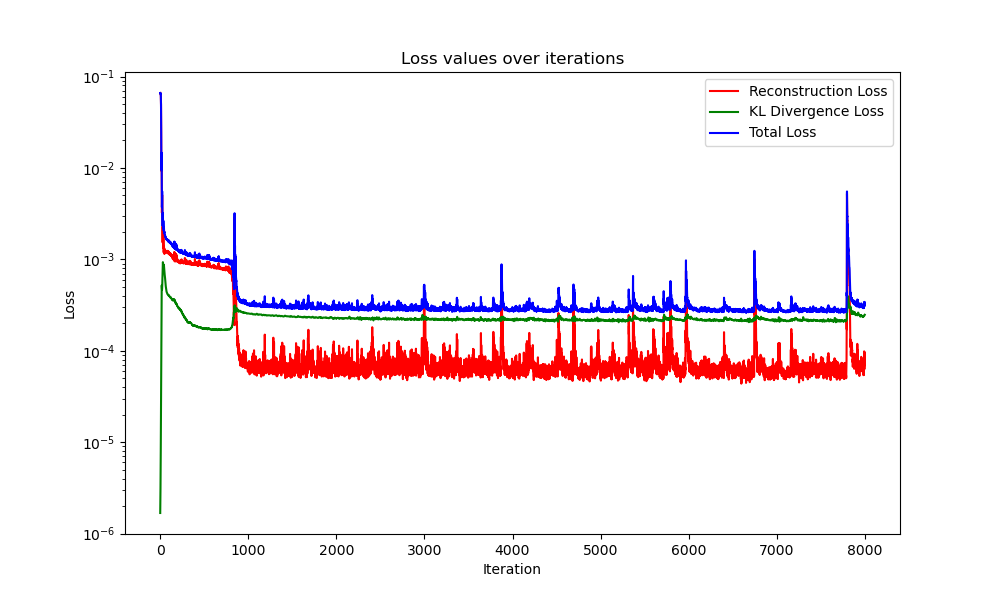
\includegraphics[width=0.8\textwidth]{../img/Figure_2.png}
    \caption{Empirical risk}
\end{figure}

\begin{figure}[H]
    \centering
    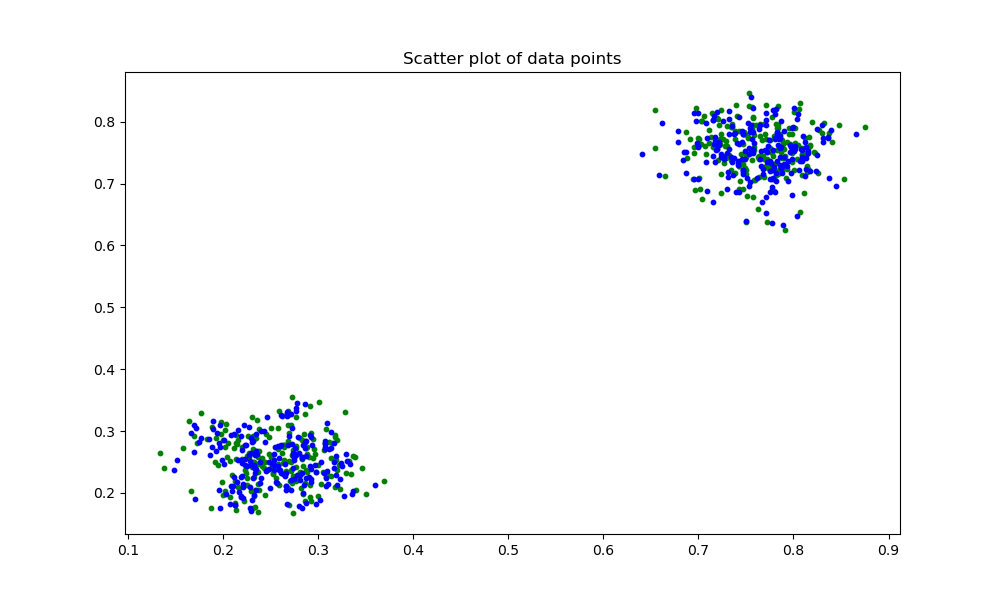
\includegraphics[width=0.8\textwidth]{../img/Figure_1.png}
    \caption{Training samples and its reconstruction}
\end{figure}

\begin{figure}[H]
    \centering
    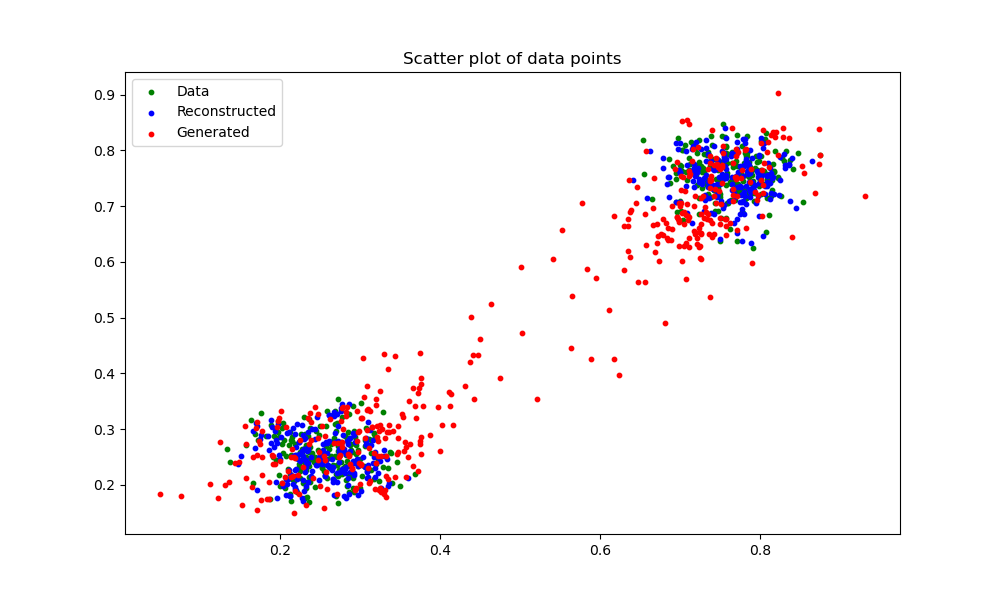
\includegraphics[width=0.8\textwidth]{../img/Figure_3.png}
    \caption{Training, reconstructed and generated samples}
\end{figure}

\end{document}
